\documentclass[../main.tex]{subfiles}
\begin{document}
\chapter{FedRAMP - Federal Risk and Authorization Management Program}
\section{Introduzione}
In questo capitolo verrà approfondito FedRAMP, il programma federale americano per la gestione del rischio e delle autorizzazioni nella cloud.
Sarà proposta un'analisi degli obiettivi del programma, specificando le problematiche in esso affrontate in relazione anche a quanto descritto nel capitolo precedente.
Verrà poi esposta la struttura del documento, dopodiché ci si concentrerà sulla struttura dello stesso approfondendo i ruoli degli attori coinvolti.
In conclusione saranno esposti i concetti di \textit{readiness} e di \textit{compliance} al programma, e sarà approfondito il ruolo dello stesso in Amazon AWS.

\section{Cos'è FedRAMP}
FedRAMP è il programma governativo americano l'applicazione del \textbf{FISMA} (Federal Information Security Management Act) nell'adozione di tecnologie cloud.
Esso propone un approccio standardizzato al \textit{security assessment}, alle autorizzazioni e al monitoraggio continuo di prodotti e servizi cloud, fornendo un insieme di requisiti di sicurezza e un programma di assessment indipendente, nato dalla collaborazione di esperti di sicurezza e di tecnologie cloud.
Le entità coinvolte nella redazione di questo programma sono state molte: la General Services Administration (GSA), il National Institute of Standards and Technology (NIST), il dipartimento di Sicurezza Nazionale (Department of Homeland Security, DHS), il dipartimento della Difesa (Department of Defense, DOD), la National Security Agency (NSA), l'Office of Management and Budget (OMB).

I \textit{cloud service provider} che vogliono offrire servizi per la pubblica amministrazione americana e gli uffici federali devono essere autorizzati tramite questo programma.
Nonostante sia stato sviluppato nel contesto USA, la dinamicità e l'elasticità di FedRAMP ne ha permesso l'adozione \textit{de-facto} anche in altre nazioni, specialmente dell'Asia orientale e del nord Europa.
\subsection{FISMA, Federal Information Security Management Act}
Il FISMA è uno standard di sicurezza, entrato in vigore come legge il 17 Dicembre 2002 come "Titolo III" dell'E-Government Act\cite{united2004information}: ciascun sistema che ospiti dati governativi deve essere autorizzato tramite il FISMA prima di essere messo in produzione.
Esso definisce tre obiettivi principali per la sicurezza dei sistemi informativi federali:
\begin{itemize}
    \item \textbf{Confidenzialità}, per garantire restrizioni autorizzate sull'accesso e la \textit{disclosure} dei dati, con l'obiettivo di proteggere la privacy ed eventuale informazioni sul proprietario odegli stessi
    \item \textbf{Integrità}, per proteggere il dato da manipolazioni o azioni distruttive e per garantire allo stesso tempo l'autenticità e la non-repudiabilità dell'informazione
    \item \textbf{Disponibilità}, per assicurare condizioni di affidabilità nell'accesso al dato
\end{itemize}

A tal fine il \textbf{NIST} ha prodotto il \textbf{Federal Information Risk Management Framework}(\textit{RMF}) il quale organizza i sistemi informatici sulla base del livello di rischio e descrive un insieme minimo di requisiti che devono essere rispettati per garantire un livello di sicurezza adeguato\cite{nist2003nist}, fornendo una metodologia per la selezione dei controlli di sicurezza e per l'esecuzione del deployment e dell'assessment.

\begin{figure}[H]
\centering
\makebox[\textwidth]{
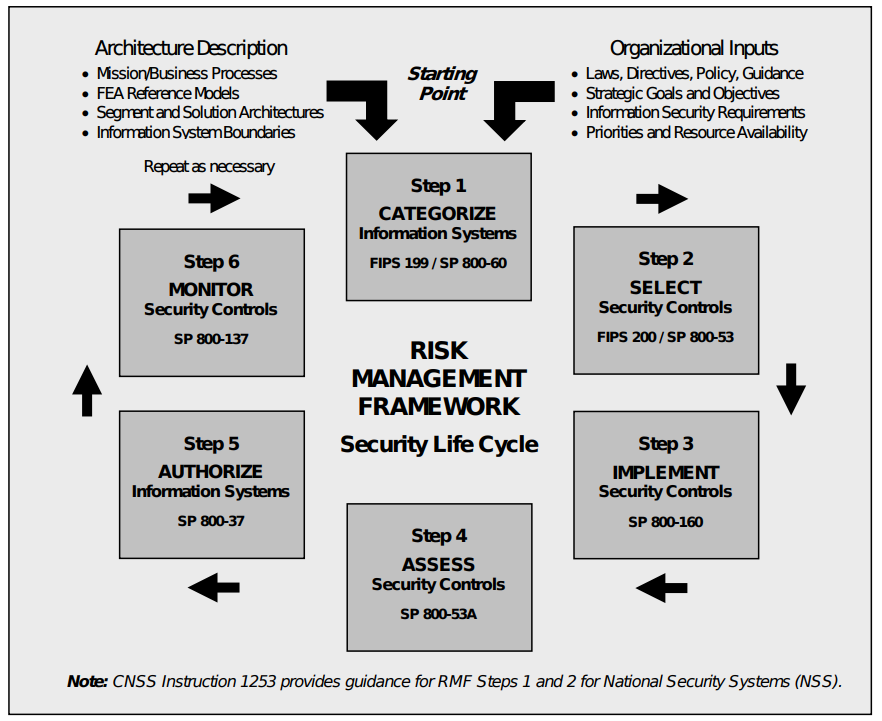
\includegraphics[width=0.8\textwidth]{immagini/risk_management_framework.png}
}
\caption{Risk Management Framework, da \cite{nist2003nist} }\label{fig:riskmanagementfw}
\end{figure}

Tramite la figura \ref{fig:riskmanagementfw} è possibile identificare le sei fasi che compongono il processo di gestione del rischio, ciclico e continuo, identificato dal framework:

\begin{itemize}
    \item \textbf{Categorizzazione del sistema informativo}, tramite i documenti FIPS\footnote{Federal Information Processing Standards} 199 e SP 800-60. Il documento FIPS 199 classifica i sistemi in base al livello di rischio, e contiene i criteri da utilizzare nella categorizzazione. Questi criteri sono basati sull'impatto potenziale di una violazione delle proprietà di confidenzialità, integrità e disponibilità sul sistema e sono: i) Rischio basso, impatto limitato, ii) Rischio medio, con serie conseguenze, iii) Rischio elevato con conseguenze gravi e catrastofiche. FIPS 199 si applica a tutti i sistemi, ad esclusione di quelli designati per l'uso della sicurezza nazionale.
    \item \textbf{Selezione dei controlli di sicurezza}, mediante i documenti FIPS 200 e SP 800-53. FIPS 200 fornisce i requisiti di sicurezza minimi (e i relativi controlli) per ogni categoria definita nel FIPS 199.
        Il documento NIST 800-53 invece definisce i controlli di sicurezza e fornisce le linee guida per scegliere i profili da impiegare per soddisfare i requisiti minimi di sicurezza, in base all'impatto del sistema. I controlli di sicurezza sono divisi in 17 famiglie e vengono divisi in tre classi (controlli di gestione, controlli operazionali e controlli tecnici). 
    \item \textbf{Implementazione dei controlli}, guidata dal documento SP 800-160
    \item \textbf{Assessment dei controlli di sicurezza}, regolato dal documento SP 800-53/A
    \item \textbf{Autorizzazione del sistema informativo}, basata sul documento SP 800-37
    \item \textbf{Fase di monitoraggio}        
\end{itemize}

\subsection{Obiettivo di FedRAMP}
L'obiettivo di FedRAMP è quindi quello di fornire un framework per semplificare il processo di autorizzazione dei servizi cloud adottati dagli enti governativi USA.
Prima dell'adozione di questo programma i produttori di sistemi e applicativi dovevano eseguire l'intero processo di autorizzazione per ciascuna delle agenzie che adottasse il sistema, così come ogni ente gestiva un processo di gestione del rischio a sé stante, anche nel caso in cui un'altra agenzia avesse già adottato servizi e misure di sicurezza analoghi. 
FedRAMP affronta la problematica nei seguenti modi:
\begin{itemize}
    \item Fornendo processi di valutazione della sicurezza e autorizzazione congiunti, basati su una serie di requisiti e controlli standardizzati, sulla base dell'impatto del sistema 
    \item Offrendo un programma di analisi della conformità in grado di produrre
    \item Strutturando un processo di analisi e valutazione della conformità condotto da Organizzazioni di terze parti approvate (3PAO), per valutare costantemente la capacità di un provider di servizi cloud (CSP) di soddisfare requisiti di sicurezza desiderati
    \item Coordinando servizi di monitoraggio continuo
    \item Fornendo pacchetti di autorizzazione composti da servizi cloud già revisionati da una Joint Authorization Board (JAB), composta da esperti di sicurezza provienienti dal DHS, dalla GSA e del DoD. 
    \item Offrendo un linguaggio standardizzato per aiutare i dipartimenti e gli enti governativi ad integrare i requisiti di FedRAMP all'interno dei processi interni
    \item Un repository di pacchetti di autorizzazione per i servizi cloud che possono essere utilizzati dal governo
\end{itemize}

L'utilizzo di un framework centralizzato ha inevitabilmente determinato un risparmio notevole anche in termini economici, sia per il governo americano, che per i cloud service provider: si stima che questo ammonti a circa \$250,000 per ciascun sistema autorizzato, per un totale di circa 160 implementazioni dello standard FISMA. Il risparmio stimato per il governo è quindi di 40 milioni di dollari.

\section{Struttura}
Il programma fornisce un percorso che i fornitori di servizi cloud possono intraprendere per ottenere una autorizzazione provvisoria, da sottoporre in una successiva fase di \textit{security assessment} che verrà poi revisionata dalla \textit{JAB}.
Mediante questo approccio preventivo è possibile quindi anticipare l'\textit{assessment} dei controlli di sicurezza e di velocizzare il processo di autorizzazione definitiva dell'applicativo o sistema cloud.


\vfill
\subsection{Attori coinvolti}
Gli attori coinvolti in FedRAMP sono quindi gli enti federali che desiderano adottare un servizio cloud, i fornitori del servizio, e le organizzazioni di terze parti che ne effettuano l'analisi della sicurezza.

\begin{figure}[H]
\centering
\makebox[\textwidth]{
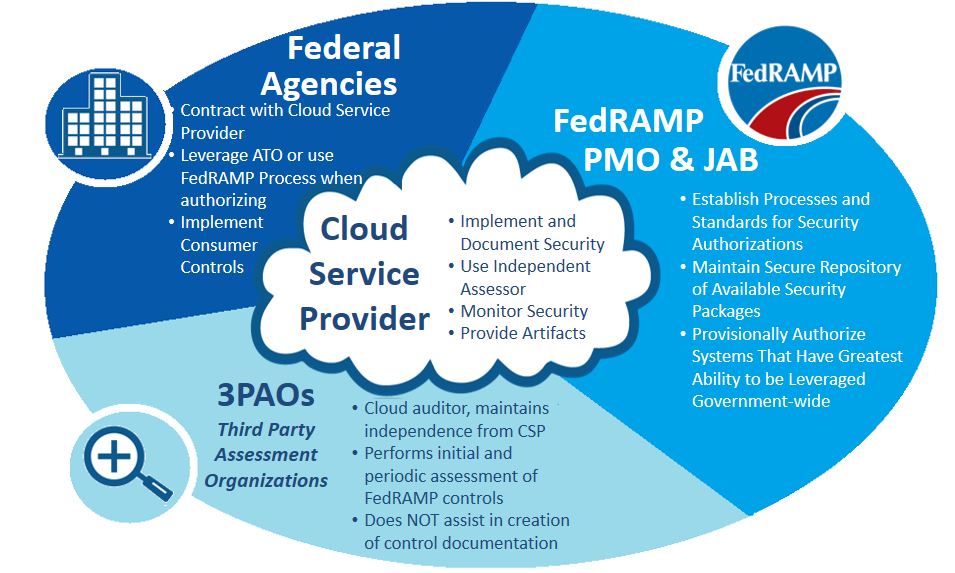
\includegraphics[width=\textwidth]{immagini/fedramp_actors.png}
}
\caption{Risk Management Framework, da \cite{} }\label{fig:fedrampactors}
\end{figure}



\subsubsection{Enti federali}
Il ruolo degli enti federali è quello di garantire che, per tutti i progetti nei quali sono coinvolte tecnologie cloud, siano rispettati i requisiti FedRAMP, venga effettuato l'assessment dei controlli di base, e siano stati forniti i template corretti.


Le agenzie devono catalogare i propri sistemi in un inventario, specificando quali di questi siano di tipo cloud e quali invece siano sistemi tradizionali. È raccomandabile avere un referente che sia preparato a rispondere a quesiti riguardanti l'implementazione dei requisiti FedRAMP.
Per facilitare ciò alcune informazioni utili potrebbero essere \textit{i) il nome del sistema cloud, ii) la descrizione del servizio fornito dal sistema, iii) il contatto dl proprietario del sistema, iv) la data di autorizzazione, v) lo stato della compliance}.


In fase di migrazione di sistemi tradizionali sul cloud, così come nell'adattamento di servizi cloud pre-esistenti a FedRAMP, è necessario che i requisiti del programma siano rispettati. Le agenzie devono quindi effetturare un'analisi approfondita delle conseguenze del cambio di tecnologia, per determinare i controlli di sicurezza aggiuntivi da effettuare.
Analogamente, gli stessi controlli di sicurezza devono interessare eventuali sistemi cloud installati ed utilizzati internamente (private-cloud). In tal caso è necessario predisporre un'analisi condotta da terze parti accreditate.
Se, invece, il fornitore del servizio è un privato e questi non ha effettuato l'assessment dei controlli di sicurezza FedRAMP, l'ente governativo è tenuto ad informare il provider e richiederne l'adeguamento immediato. 

Le agenzie, sulla base di specifiche esigenze, possono sottomettere eventuali controlli aggiuntivi rispetto a quelli basilari; questi devono devono essere adeguatamente documentati e motivati. Gli altri enti possono poi decidere di adottare questi controlli.
Allo stesso modo, come già trattato, le agenzie possono riutilizzare autorizzazioni emesse per altri enti.

Sulla base del E-Government Act del 2002 (Titolo III, Sezione 3544), le agenzie devono inoltre effettuare analisi del rischio periodiche, valutando l'impatto di eventuali violazione della confidenzialitàe dell'integrità dei dati.

Uno degli obiettivi della piattaforma presentata in questo lavoro di tesi, è quello di fornire uno strumento a supporto delle agenzie federali per la gestione della sicurezza degli asset inventariati (sistemi tradizionali e cloud), fornendo sia meccanismi di \textit{auto-discovery} degli stessi (ad esempio mediante l'integrazione con le API dei cloud service provider, oppure tramite la scansione delle reti locali), sia un processo di monitoraggio continuativo della stato della compliance.

\subsubsection{Organizzazioni di terze parti (3PAO)}
Affinché un servizio cloud possa essere autorizzato da FedRAMP, è necessario che un'organizzazione di terze parti ne analizzi la sicurezza mediante l'esecuzione dei controlli standardizzati nel documento NIST 800-53.
Per ottenere l'abilitazione ad effettuare queste analisi, l'organizzazione può decidere di iniziare un percorso di accreditamento, il cui obiettivo è quello di garantire che che le analisi siano effettuate in maniera consistente, dettagliata e indipendente.
A tal fine, l'organizzazione deve inviare sottomettere del materiale in grado di dimostrare di essere in grado sia di eseguire analisi tecniche adeguate ai livelli attesi, sia di avere competenza nella gestione dei processi di \textit{compliance}.
Questi criteri vengono certificati dalla \textit{American Association for Laboratory Accreditation (A2LA)} che, dopo aver verificato le effettive competenze tecniche in capo alll'organizzazione, effettua un processo di controllo della conformità rispetto allo standard ISO/IEC 17020 (Disposizioni per la transizione degli accreditamenti degli Organismi di ispezione (OdI)).


Il testing della sicurezza nei confronti dei fornitori di servizi deve essere effettuato in modo equo, tramite controlli scelti sulla base della loro categoria di sensibilità. La periodicità è annuale, e la stessa organizzazione non può effettuare una scansione per due anni consecutivi.
In alcuni casi può essere necessario eseguire test automatici come utenti autenticati e con pieni privilegi, in modo da poter determinare con precisione le vulnerabilità e il relativo impatto sul sistema. Solo in questo modo, infatti, è possibile avere una visione globale del sistema (ad es. accedere al registro di sistema di Windows, agli attributi dei file di sistema, ai pacchetti e alle patch effettivamente installate). L'utilizzo di un utente con privilegi limitati può restituire sia falsi positivi (ad esempio nel caso di un test di scrittura su directory interne al sistema eseguito in un ambiente \textit{chroot}) e falsi negativi (in caso di assunzioni derivate dall'impossibilità per l'utente di leggere determinati parametri).
Eventuali analisi del codice, invece, sono demandate al \textit{cloud service provider}.

Per guidare questo processo in modo standard, FedRAMP fornisce vari template, scaricabili dal sito ufficiale:
\begin{itemize}
    \item \textit{Security Assessment Plan Template}, il cui scopo è quello di descrivere il piano per l'analisi della sicurezza. Prima di redigere questo documento, l'organizzazione deve incontrarsi col fornitore di servizi cloud per discutere i test da eseguire. Eventuale supporto può essere erogato dall'\textit{Information System Security Officier} di FedRAMP.
    \item \textit{Security Assessment Test Cases}, in cui vengono descritti i casi di test sulla base del documento NIST 800-53A; alcuni di questi, tuttavia, differiscono poiché sono stati adattati al contesto \textit{cloud}. Nel caso in cui l'organizzazione debba implementare versioni alternative dei controlli di sicurezza, è necessario che i casi di test vengano scritti in modo idoneo ad attestarne l'efficacia.
    \item \textit{Security Assessment Report}, assiste la parte di reportistica, il cui obiettivo è quello di dettagliare l'analisi eseguita sui sistemi del fornitore di servizi cloud, riportando le evidenze trovate, le possibili operazioni di mitigazione e le eventuali raccomandazioni.
\end{itemize}

Il sistema progettato nell'ambito di questo progetto di tesi, mira a diventare uno strumento di supporto delle organizzazioni di terze parti.
Uno dei possibili sviluppi in tal senso, potrebbe consistere nell'integrazione dei template presentati in questa sezione all'interno della piattaforma realizzata, in modo da poter guidare l'intero processo di \textit{security assessment}, e consentire anche ad organizzazioni differenti di mantenere una cronologia delle analisi svolte su uno specifico servizio cloud. 

\subsubsection{Fornitori di servizi cloud}
Il \textit{cloud service provider} può essere sia un'entità di terze parti commerciale che un altro ente governativo od agenzia. La sua responsabilità è quella di implementare i controlli di sicurezza, di assumere un'organizzazione di terze parti indipendente che effettui l'assessment annuale e di effettuare tutte le procedure per la creazione e la manutenzione delle proprie autorizzazioni.

Le modalità con cui un fornitore di servizi può essere autorizzato sono tre:
\begin{itemize}
    \item Il provider può inviare la documentazione appropriata al PMO (ufficio di gestione del programma FedRAMP) e alla Joint Advisory Board, che possono erogare un'autorizzazione provvisoria (P-ATO, Provisional Authorization to Operate) 
    \item Il provider può inviare la documentazione appropriata al PMO e ad un'agenzia, che può erogare un'autorizzazione ad operare (ATO, Authorization to Operate). Come già spiegato, un'altra agenzia può utilizzare poi la stessa autorizzazione, abbreviando i tempi di approvazione.
    \item Il provider può inviare la documentazione per intraprendere autonomamente un percorso di tipo "CSP supplied". In tal caso, dovrà assumere una organizzazione di terze parti che ne analizzi la sicurezza.
\end{itemize}

Quindi, affinché un sistema cloud sia conforme con FedRAMP:
\begin{itemize}
    \item deve essere stato creato e sottomesso un pacchetto, utilizzando i template idonei
    \item deve essere stato eseguito l'assessment, da parte di un'organizzazione di terze parti accreditata e indipendente, mediante l'esecuzione dei controlli di sicurezza relativi al livello di sensibilità del sistema (basso o medio, in quanto i sistemi ad alta sensibilità non sono supportati dal programma e devono essere gestiti separatamente).
    \item l'assessment deve aver restituito risultati positivi, attestando che i requisiti di sicurezza siano effettivamente verificati
    \item deve essere stata erogata un'autorizzazione ad operare, provvisoria o definitiva
\end{itemize}

\section{FedRAMP readiness}

Il provider che vuole partecipare a FedRAMP deve innanzitutto soddisfare una serie di requisiti di \textit{readiness}:
\begin{enumerate}
    \item Essere in grado di trattare eventuali processi forensi elettronici e contenziosi 
    \item Essere in grado di definire e descrivere chiaramente i confini del proprio sistema
    \item Identificare le responsabilità del cliente e le azioni che questo deve compiere per implementare i controlli di sicurezza
    \item Fornire un meccanismo di identificazione e autenticazione a due fattori per l'accesso via rete agli account privilegiati
    \item Fornire un meccanismo di identificazione e autenticazione a due fattori per l'accesso via rete agli account non privilegiati
    \item Fornire un meccanismo di identificazione e autenticazione a due fattori per l'accesso locale agli account privilegiati
    \item Avere la possibilità di eseguire analisi del codice per le soluzioni software proprietarie
    \item Avere protezioni di confine garantendo isolamento logico e fisico degli asset
    \item Avere l'abilità di rimediare a situazioni di rischio elevato entro i 30 giorni (90 giorni per le situazioni di rischio moderato)
    \item Fornire un inventario e configurazioni standard per tutti i dispositivi
    \item Avere meccanismi di sicurezza che impediscano la fuoriuscita di informazioni nell'utilizzo di mezzi di comunicazione condivisi
    \item Adottare meccanismi di crittografia per preservare la confidenzialità e l'integrità dei dati trasmessi sulla rete
\end{enumerate}


Se queste condizioni sono rispettate, è possibile sottomettere un modulo di richiesta di ammissione al programma, disponibile online sul sito web di FedRAMP. A questo seguirà una notifica automatica all'ufficio di gestione del programma e alla \textit{Joint Advisory Board}.
In questo modulo il provider fornisce informazioni sul proprio sistema, categorizzandolo sulla base delle direttive contenute nel documento NIST SP 800-60 V2, e decide la \textit{baseline} dei controlli di sicurezza da implementare in base alla sensibilità del sistema (bassa o media).

A seguito di una revisione della \textit{readiness} da parte dell'ufficio di gestione del programma, sarà possibile avviare il processo di richiesta dell'autorizzazione provisoria (P-ATO): il \textit{cloud service provider} deve quindi ricercare ed assumere un'organizzazione di terze parti, tra quelle specificate sul sito di FedRAMP.

Oltre alle finalità precedentemente esposte, il prodotto sviluppato in questo lavoro di tesi punta a supportare il processo di verifica dei requisiti tecnici richiesti per la \textit{readiness}. In particolare si vogliono fornire controlli di sicurezza per i punti 3, 4, 5, 11 e 12.
I restanti requisiti, di carattere meramente procedurale, saranno invece implementati separatamente sotto forma di questionario.



\section{Documenti aggiuntivi}

5.3. After Acceptance into the FedRAMP Program
After acceptance into the FedRAMP JAB Provisional Authorization process, there are certain documents requiring submission.  The FedRAMP PMO created templates for documents that the CSP must edit and modify based on the security controls implemented in its system.  All templates are available on the FedRAMP website.  Guidance on how to fill out the various templates and develop the required documents are described in the sections that follow.  




After acceptange in to the program, there are other documents that have to be submitted for which templates are provided.
Those are discussed in the next slides.



FIPS 199
Allow the  CSPs to categorize and record the sensitivity level of the system according to the NIST SP 800-60 Revision 1 Volume 2.
IaaS and PaaS providers must select information types from section C.3.5

E-Authentication Template
An e-Authentication template is provided for performing an e-Authentication analysis. The objective is to ensure that the CSP has implemented technical solutions that matches the sensitivity of the system and the data it stores and the processes.
The guidance document is NIST SP 800-63, Revision 1, Electronic Authentication Guidance.
e-Authentication template is provided on FedRAMP’s website.

Privacy threshold Analysis & Privacy impact assessment
CSPs are required to fill out a Privacy Threshold Analysis (PTA).
FedRAMP provides a PTA/PIA template, that consists of four short questions designed to determine if the system qualifies as a Privacy Sensitive System. If so, then a Privacy Impact Assessment (PIA) is also required.
In accordance with NIST SP 800-144, organizations are ultimately accountable for the security and privacy of data held by a cloud provider on their behalf.
CSPs must consider whether their security controls (for their own support staff) use PII for any authentication mechanisms (e.g. fingerprint scanners, hand scanners, iris scanners). If the CSP system requires PII from agency customers, for example, to enroll users in authentication mechanisms, then the impending collection of that PII on first use by agency customers should
be made known.
When performing the independent security assessment, the 3PAO will review the PTA and/or PIA to make certain determinations and findings that are incorporated into the Security Assessment Report (SAR).

CTW Template

The purpose of the Control Tailoring Workbook (CTW) template is to summarize the exception scenarios of the service offering for prospective agency customers. This template is completed after the System Security Plan has been completed, and must be consistent with information found in the System Security Plan.

CIS Template
Complete the Control Implementation Summary (CIS) template to indicate the implementation status of the controls for the system.
CSPs need to indicate in the CIS the entity responsible to implement and manage the control. In some cases, implementation and management of a control may require joint ownership by the CSP and the customer agency
The CIS is a living document and updates are expected throughout the development of the System Security Plan.

User guide
CSPs must provide a User Guide that explains how prospective users (government agencies) will use the system. If the system has a self-service control panel, the User Guide must explain clearly how to use the control panel. Submit the User Guide with the System Security Plan.

Components, boundaries, architecture
The System Security Plan template documents and describes how all required security controls are implemented. 
The CSP system likely has multiple components. Each component needs to be named and described in Section 9.2 of the System Security Plan. Wherever possible, use component names that are already familiar and used within the organization. Components may be described by a unique name (e.g. “Home Base”) or by functionality (e.g. “the Hypervisor”).
Discussing virtualization
This section includes general guidance on discussing virtualization in System Security Plans.
There are numerous ways that virtualization can be implemented, and many different virtualization products.
The FedRAMP PMO does not make recommendations on virtualization models or products. Whatever virtualization architecture model is used, CSP documentation in all aspects must be clear about
which components are parts of the physical host system
which components are parts of virtual abstraction layers
When discussing the functionality of different components, indicate whether the component is
a standard host operating system
guest (virtual) operating system.
For each physical host that provides the capability to implement guest systems, discuss whether the virtualization technique is based on:
hosted virtualization
bare metal virtualization

Guest operating systems can be deployed in several ways:
the CSP provides a self-service menu driven control panel where customers can setup and configure their own virtual machines within a controlled environment
the CSP installs and configures unique virtual machines instances directly for the customer thereby eliminating the need for a self-service portal. 
When discussing administration, access control, and configuration settings of virtual machines, CSPs need to be clear about whether their service offers a self-serve solution or a CSP administered solution.
The roles and authorizations associated with both of these solutions must be detailed in the System Security Plan (Table 9-1) User Roles and Privileges.
Network components can also be virtualized. When discussing a network component (or device) that is a virtual component, be clear about the fact that the item discussed is virtual and not physical (VLANs, Virtual Ethernet Modules, Virtual Firewalls, Virtual Switches, Virtual Distributed Switches, Virtual Security Gateways, Virtual Routers, NAT Virtual Interfaces).

Discussing virtualization - boundaries and inherited controls
When describing the boundaries of the cloud system, it is important to accurately and clearly articulate where the cloud service layers begin and end.
If a PaaS service provider is building its service on top of an IaaS service provider, the PaaS provider needs to ensure that their security control boundaries begin where the IaaS security control boundaries end. Alternately, a SaaS provider must understand where the PaaS security control boundaries end.
The security controls for an upper layer service needs to begin where the lower layer security controls end.
There are many possible configurations for layering security and FedRAMP does not make recommendations on specific service models.
When discussing boundaries, include information on how different tenants are separated from each other in a multi-tenant environment.


Questions to consider when describing boundaries:
Will the boundaries leverage any existing Provisional Authorizations?
What is the definition of a tenant?
For the service offering, will multiple tenants share the same VLAN(s)?
Are there controls that prevent VLAN hopping?
Are virtual machine zones on unique network segments isolated?
Are separate physical network adapters used to isolate virtual machine zones?
Is layer-2 isolation performed?
Is isolation through traffic encapsulation used?
Do port groups define any boundaries?
If port groups are used, are they all in the same layer-2 domain or do they span multiple
layer-2 domains?
Are multiple Network Interface Cards (NICs) bonded together?
How do firewalls provide isolation between tenants?

Questions to consider when describing boundaries:
How does router ACLs provide isolation between tenants?
Are IPsec tunnels used to define boundaries?
Is sharding used?
Are network filters used that control what packets are sent to or from a virtual machine?
Are network zones used? If yes, how are zones defined?
Will U.S. federal agencies be multi-tenanted with non-government entities?
Are NAT virtual interfaces (NVI) or domain specific NAT configurations used?
How does NAT play a role in containing network traffic within the boundary?
What kind of NAT is used? (e.g. static, dynamic, overloading, overlapping)
Are NAT IP pools used?
Are geo IP location boundaries used?
Define the geographic location (City, State) where customer data is stored?
Will it be possible for agency tenants to know the geographic location (City, State) where
their data is stored?

Discussing live migrations

Live migrations of virtual machines have the potential to confuse a common understanding of the information system boundaries. Therefore, when describing boundaries, it is important to discuss the live migration strategy for the information system. Live migrations have the ability to move an entire virtual machine to another host or instead, move a virtual machine’s data store (configuration file and virtual disks) to another physical host without actually moving the virtual machine. Complicating this, it is also possible to move and store a virtual machine’s configuration files, and disks in separate locations. The FedRAMP PMO does not make recommendations on live migration strategies. Whatever the live migration strategy is, be clear as to how live migrations are managed.
IP addresses declared within the boundary must remain protected by the security controls noted in the System Security Plan even if the IP addresses are moved around.
Questions to consider in the discussion of live migration:
Are live migrations performed manually, or scheduled and automated?
If live migrations are automated, what are the rules that govern the migration?

Discussing storage components

In the description of system components, include information about storage components that are inside the boundary. If using a fiber channel storage array, insert a diagram that shows how the storage connects to the fiber channel fabric and include the switches in the diagram.
Questions to consider when describing storage components:
Does the system use Direct Attached Storage (DAS), Network Attached Storage (NAS), or Storage Area Networks (SANs)?
If using a SAN, what is used to connect hosts in a cluster (fiber channel or iSCSI)?
Which fiber channel or iSCSI connections are considered within the boundary?
Are different types of storage devices used on different network segments?
Are clusters used?
How many hosts are on a cluster and which clusters are in the boundary?
Do the storage devices use a multipath environment?
Are the storage devices set up to be persistent or non-persistent?

Data flow Diagram

Describes how network traffic flows through the platform and offering.
A data flow diagram focuses more on the direction of the network traffic and less on the actual network topology. However, certain components of the system’s network topology need to be included to illustrate the direction that the network traffic flows through the system.




\section{Controlli di sicurezza per la conformità - NIST 800-53}
\subsection{Categorie dei controlli}
\subsection{Controlli procedurali}
AC-1,AC-2(a),AC-2(b),AC-2(c),AC-2(d),AC-2(e),AC-2(f),AC-2(g),AC-2(h),AC-2(i),AC-2(j),AC-2(7)(a),AC-5,AC-6(1),AC-8(b),AC-11(b),AC-17(a),AC-17(b),AC-17(4),AC-17(5),AC-17(6),AC-19(b),AC-19(1),AC-19(2),AC-19(3),AC-19(4)(a),AC-19(4)(b),AC-20(a),AC-20(b),AC-20(1)(a),AC-20(1)(b),AC-20(2),AC-21(a),AC-21(b),AC-22(a),AC-22(b),AC-22(c),AC-22(d),AC-22(e),AU-2(b),AU-6(a),AU-6(b),AU-6(3),CA-1(a),CA-1(b),CA-2(a),CA-2(b),CA-2(c),CA-2(d),CA-2(1),CA-2(2),CA-3(a),CA-3(b),CA-3(1),CA-3(2),CA-5(a),CA-5(b),CA-6(a),CA-6(b),CA-6(c),CM-3(a),CM-3(b),CM-3(c),CM-3(d),CM-3(e),CM-3(f),CM-3(4),CM-7(3),IA-1(a),IA-1(b)
\subsection{Controlli automatizzabili}
\subsubsection{i}

AC-3(4),AC-14(a),AC-14(b),AC-14(1),AC-17(c),AC-17(d),AC-17(e),AC-18(b),AC-18(c),AC-18(4),AC-19(c),AC-19(f),AC-19(g),AU-3,AU-8,AU-9(4)(b),AU-12(b),CM-8(3)(a),IA-2,IA-5(e),IA-6,IA-8" 

AC-2(1),AC-7(a),PM-11,PM-10,PM-9,PM-8,PM-7,PM-6,PM-5,PM-4,PM-3,PM-2,PM-1,AC-17(3),AC-18(a),AC-18(b),AC-18(5),AC-21(1),CP-10(2),AT-1(a),AT-1(b),AT-2,AT-3,AT-3(2),AT-4(a),AT-4(b),AT-2,AT-2(1),AT-3,AT-3(1),AT-3(2),AT-5,AU-1(a),AU-1(b),AU-2(3),AU-6(1),AU-6(3),AU-7,AU-7(1),CA-7(a),CA-7(b),CA-7(c),CA-7(d),CA-7(1),CA-7(2),CM-1(a),CM-1(b),CM-2,CM-2(1)(a),CM-2(1)(b),CM-2(1)(c),CM-2(2),CM-2(5)(a),CM-2(5)(b),CM-3(2),CM-4,CM-4(2),CM-5,CM-5(2),CM-5(5)(b),CM-6(a),CM-6(b),CM-6(c),CM-6(1),CM-7(1),CM-8(a),CM-8(b),CM-8(c),CM-8(d),CM-8(e),CM-8(1),CM-8(4),CM-8(5),CM-8(6),CM-9(a),CM-9(b),CM-9(c),CP-1(a),CP-1(b),CP-2(a),CP-2(b),CP-2(c),CP-2(d),CP-2(e),CP-2(f),CP-2(1),CP-2(2),CP-3,CP-4(a),CP-4(b),CP-4(1),CP-6,CP-6(1),CP-6(2),CP-7(a),CP-7(b),CP-7(1),CP-7(2),CP-7(3),CP-7(5),CP-8,CP-(8)(1)(a),CP-8(1)(b),CP-8(2),CP-9(a),CP-9(b),CP-9(c),CP-9(d),CP-9(1),CP-9(3),CP-10,CP-10(2),CP-10(3),IA-4(a),IA-4(b),IA-4(c),IA-4(d),IA-4(e),IA-4(4),IA-5(a),IA-5(d),IA-5(3),IA-5(6),IA-5(7),IR-1(a),IR-1(b),IR-2(a),IR-2(b),IR-3,IR-4(a),IR-4(b),IR-4(c),IR-4(1),IR-6,IR-7,IR-7(1),IR-7(2),IR-8(a),IR-8(b),IR-8(c),IR-8(d),IR-8(e),MA-1(a),MA-2(a),MA-2(b),MA-2(c),MA-2(d),MA-2(e),MA-2(1),MA-3,MA-3(1),MA-3(2),MA-3(3),MA-4(a),MA-4(b),SI-1(a),SI-1(b),SI-2(a),SI-2(b),SI-2(c),SI-3(a),SI-3(b),SI-3(c),SI-3(d),SI-3(1),SI-1(2),SI-1(3),SI-4(a),SI-4(b),SI-4(c),SI-4(d),SI-4(e),SI-4(2),SI-4(4),SI-4(5),SI-4(6),SI-5(a),SI-5(b),SI-5(c),SI-5(d)


\section{FedRAMP in Amazon AWS}
Certificazioni di conformità di AWS
Per visualizzare i report di conformità AWS, utilizza AWS Artifact, un portale self-service per l’accesso on demand. Per istruzioni sull'utilizzo di Artifact, guarda il nostro video sulla home page Artifact. In caso di domande, compila il modulo seguente per essere contattato da un rappresentante aziendale di Amazon Web Services.

 AWS ha soddisfatto i controlli di sicurezza previsti dal programma FedRAMP (basati su NIST SP 800-53), ha impiegato modelli predefiniti per i pacchetti di sicurezza pubblicati nel repository FedRAMP, ha sostenuto la valutazione di un'entità di controllo indipendente accreditata e soddisfa i requisiti di monitoraggio continuo del programma FedRAMP. I sistemi conformi sono i seguenti:

AWS GovCloud (US) ha ricevuto un'autorizzazione provvisoria del Joint Authorization Board (JAB P-ATO) e diverse autorizzazioni operative per il livello di impatto High. I servizi coperti dall'autorizzazione provvisoria del Joint Authorization Board nella regione AWS GovCloud (US) sono disponibili nella pagina relativa alla copertura di conformità dei servizi AWS. Per consultare un elenco completo delle agenzie che hanno rilasciato autorizzazioni operative per la regione AWS GovCloud (US), visita la pagina FedRAMP Compliant Systems.

Regioni AWS Stati Uniti occidentali/orientali: hanno ricevuto diverse autorizzazioni operative per il livello di impatto Moderate. I servizi coperti dalle autorizzazioni provvisorie per le regioni AWS Stati Uniti occidentali/orientali sono disponibili nella pagina relativa alla copertura di conformità dei servizi AWS. Per consultare un elenco completo delle agenzie che hanno rilasciato autorizzazioni operative per le regioni AWS Stati Uniti occidentali/orientali, visita la pagina FedRAMP Compliant Systems.

La conformità con il programma FedRAMP farà aumentare i costi dei servizi AWS?
No, la conformità al programma FedRAMP da parte di AWS non provocherà alcun aumento dei costi in alcuna regione.

Quali regioni AWS sono coperte?
AWS ha ottenuto due Agency ATO FedRAMP separate, una a copertura della regione AWS GovCloud (Stati Uniti), l'altra delle regioni Stati Uniti occidentali e orientali.

I clienti di AWS possono richiedere l'accesso ai pacchetti di sicurezza FedRAMP di AWS tramite il FedRAMP PMO o all'account manager delle vendite di AWS.

Le agenzie governative statunitensi possono richiede l'accesso al pacchetto di sicurezza FedRAMP di AWS tramite il FedRAMP PMO compilando un modulo di richiesta di accesso al pacchetto e inviandolo all'indirizzo info@fedramp.gov, oppure contattando l'account manager delle vendite di AWS.

I partner di AWS e i clienti potenziali possono anche richiedere l'accesso al pacchetto di sicurezza FedRAMP di AWS per i partner contattando l'account manager delle vendite di AWS.

Un funzionario autorizzato di un'agenzia può impiegare uno dei pacchetti di sicurezza FedRAMP di AWS ed esaminarne la documentazione per decidere in base ai rischi di assegnare un'autorizzazione operativa (ATO) ad AWS. Le agenzie sono responsabili per il rilascio delle autorizzazioni operative in AWS e in generale per le autorizzazioni dei componenti dei loro sistemi non coperte dall'autorizzazione operativa di AWS. Per ulteriori informazioni sul modello di responsabilità condivisa di AWS, contatta l'account manager delle vendite di AWS.

Impiegando le funzionalità di sicurezza offerte da AWS e dall'ecosistema di fornitori, potrai controllare e monitorare la creazione di sistemi disponibili in modo che integrino le policy di gestione della sicurezza, della privacy e o del rischio dell'agenzia.

Scoprilo leggendo cosa sono stati in grado di realizzare clienti, partner e integratori di sistemi grazie ad AWS:

Blog

Appian Cloud sfrutta l'infrastruttura di Amazon Web Services e l'autorizzazione FedRAMP. Leggi tutto

Casi di studio AWS

Dipartimento di Stato degli Stati Uniti

US Food and Drug Administration (FDA)

US Centers for Disease Control and Prevention (CDC)

NASA/JPL: Desert Research and Training Studies

NASA/JPL e Amazon SWF

NASA/JPL: la missione Curiosity su Marte

All'interno del documento Concept of Operations (CONOPS) del programma FedRAMP, quando un'autorizzazione è stata assegnata, il livello di protezione di un CSP viene monitorato secondo il processo di valutazione e autorizzazione. Per ottenere una nuova autorizzazione di una ATO FedRAMP da un anno all'altro, i CSP devono monitorare i propri controlli di sicurezza, effettuarne delle valutazioni periodiche e dimostrare che la sicurezza della loro offerta di servizi mantiene sempre un livello accettabile. La valutazione della continuità della conformità è responsabilità delle agenzie federali che impiegano il programma di monitoraggio continuo FedRAMP, nonché dei funzionari autorizzati e relativi team. I funzionari autorizzati e i relativi team esamineranno gli artefatti forniti tramite il processo di monitoraggio continuo FedRAMP di AWS, oltre alle prove di implementazione di controlli specifici della singola agenzia che fanno parte dei requisiti esterni ai controlli FedRAMP, in modo continuo. Per ulteriori informazioni, consulta la policy o il programma di sicurezza dei sistemi informatici della tua agenzia.


\end{document}
